\documentclass[preview]{standalone}

\usepackage{amsmath}
\usepackage{amssymb}
\usepackage{stellar}
\usepackage{bettelini}

\hypersetup{
    colorlinks=true,
    linkcolor=black,
    urlcolor=blue,
    pdftitle={Biologia},
    pdfpagemode=FullScreen,
}

\begin{document}

\title{Biologia}
\id{biologia-membrane}
\genpage

\begin{snippetdefinition}{membrana-definizione}{Membrana}
    Le \textit{membrane} sono dei fosfolipidi con una code e una testa idrofila.
\end{snippetdefinition}

\plain{Questi fosfolipidi si attraggono per polarità e possono formare le seguenti composizioni}

\begin{snippet}{membrana-illustration}
    \begin{center}
    \begin{figure}[h]
        \centering
        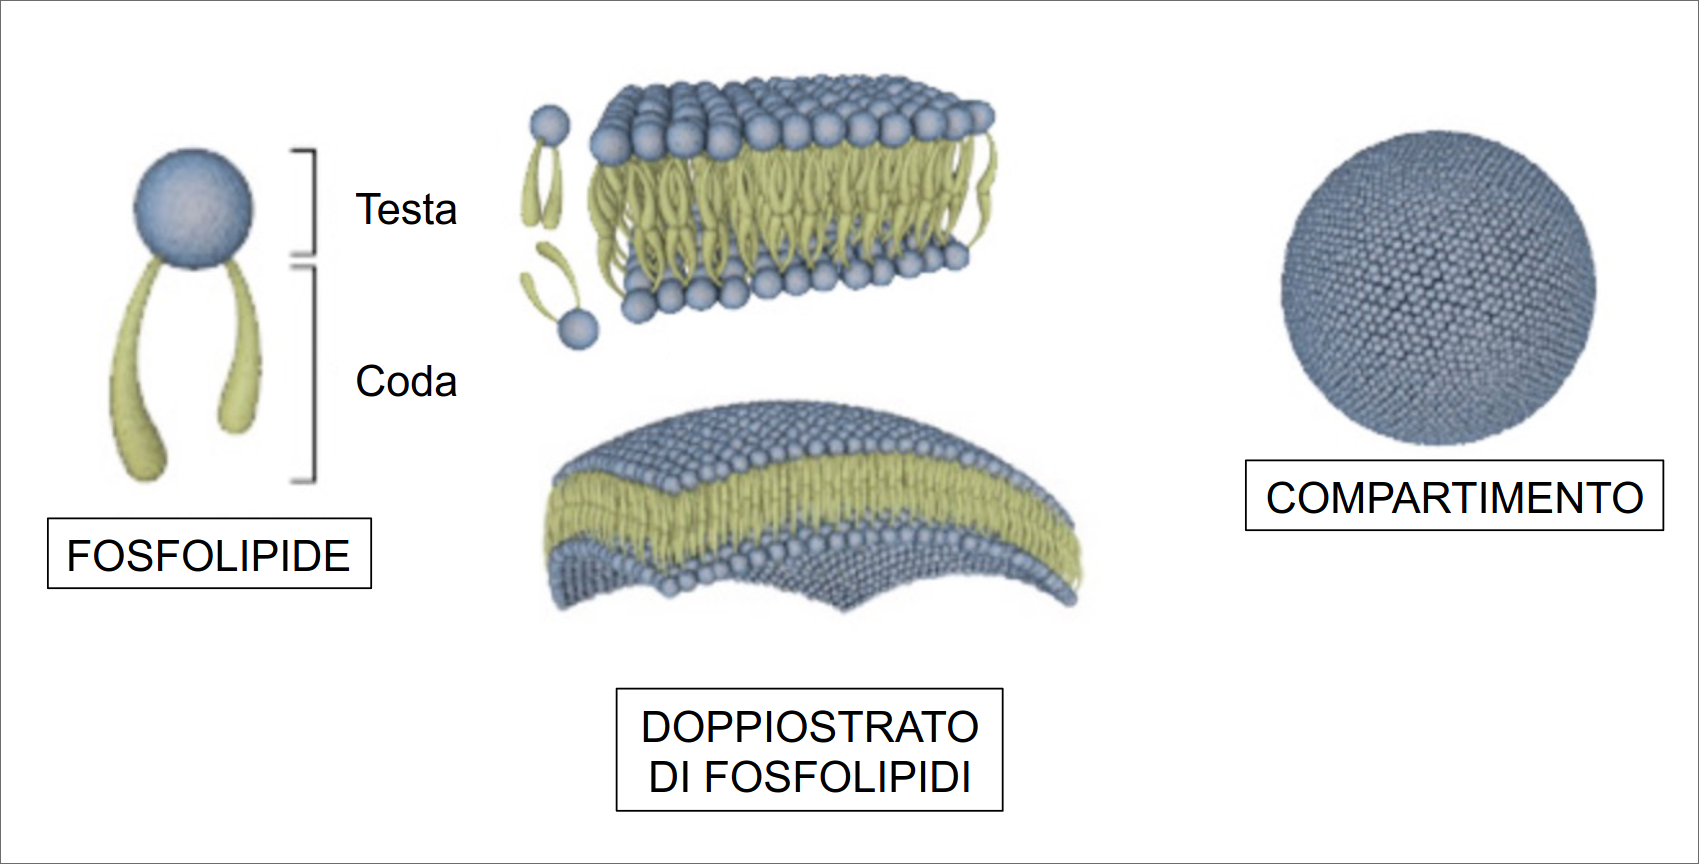
\includegraphics[width=\textwidth]{./resources/membrana.png}
    \end{figure}
    \end{center}
\end{snippet}

\plain{Le sostanze idrofile (steroidi, grassi, etc.) vengono trasportati nel sangue}

\section{Proteine di membrana}

\begin{snippetdefinition}{gradiente-concentrazione-definizione}{Gradiente di concentrazione}
    Il \textit{gradiente di concentrazione} è un regolare incremento o diminuzione della concentrazione di una sostanza. Quando è presente un gradiente di concentrazione, gli ioni o le altre sostanze coinvolte tendono a muoversi spontaneamente dalla zona di concentrazione maggiore a quella di concentrazione minore.
\end{snippetdefinition}

\plain{Le principali tipologie di proteine che vengono incastrate nelle membrane sono:}

\begin{snippetdefinition}{proteina-trasporto-definizione}{Proteina di trasporto}
    Una \textit{proteina di trasporto} (canale) è una proteine di membrana che forma un tunnel sempre aperto.
\end{snippetdefinition}

\plain{Ogni canale non è direzionale ed ogni canale è specifico per un certo soluto.}

\begin{snippet}{proteine-mem-illustration}
    \begin{center}
    \begin{figure}[h]
        \centering
        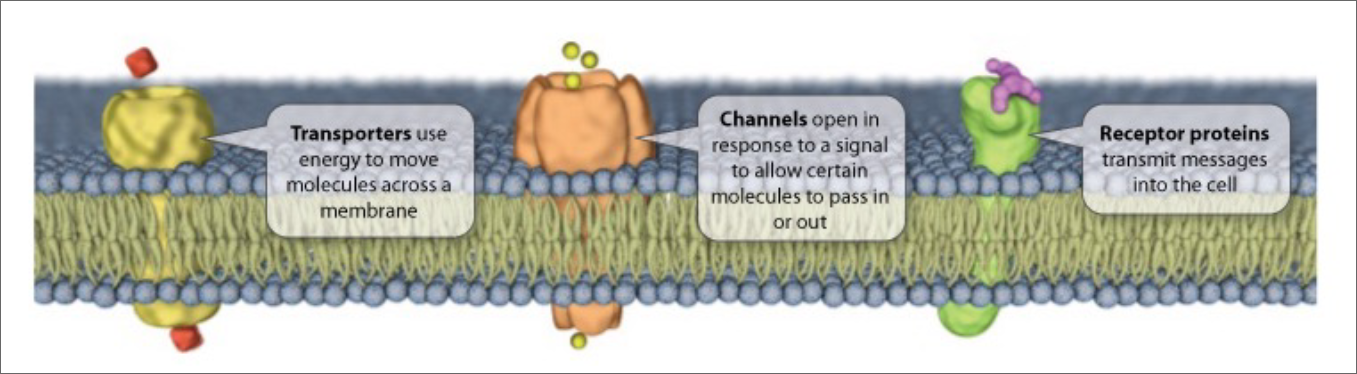
\includegraphics[width=\textwidth]{./resources/proteine_mem.png}
    \end{figure}
    \end{center}
\end{snippet}

\begin{snippet}{4379597a-31a3-45ff-8799-dc834610fa2c}
    Tuttavia, siccome le cellule necessitano un ambiente interno diverso da quello esterno,
devono andare contro il gradiente di concentrazione.
Per risolvere questo problema vengono utilizzati i trasportatori.
\end{snippet}

\begin{snippetdefinition}{trasportatore-definizione}{Trasportatore}
    Un \textit{trasportatore} è una proteina che sposta una sostanza contro il gradiente.
\end{snippetdefinition}

\plain{Ogni tipo di trasportatore è specifico ad un tipo di sostanza.
Il trasportatore sposta quindi una sostanza da dove ce n'è poca a dove ce n'è tanta (mediante energia).}

\begin{snippetdefinition}{ricettore-definizione}{Ricettore}
    Un \textit{ricettore} è una proteina che comunica dei messaggi alla cellula.
\end{snippetdefinition}

\begin{snippetexample}{ricettore-example}{Ricettori}
    Un ricettore potrebbe per esempio comunicare il segnale della presenza di un agente patogeno.
\end{snippetexample}

% todo fare 2 definitions
\begin{snippet}{77bc0611-e850-4247-884d-62d8441cdfa7}
    Alcune molecole possono passare direttamente attraverso la membrana, come per esempio l'azoto, l'ossigeno, acqua e glicerolo.
    Questo movimento è detto diffusione semplice nei fosfolipidi. Chiaramente, la cellula non può controllare queste sostanze.

    Le molecole grandi e ioni non passano per i fosfolipidi senza un canale (diffusione facilitata).

    % grandiente elttrochimico con polarità
\end{snippet}

\begin{snippetdefinition}{trasporto-attivo-primario-definizione}{Trasporto attivo primario}
    Il \textit{trasporto attivo primario} è un trasporto grazie ad un trasportatore e all'ATP.
\end{snippetdefinition}

\begin{snippet}{8cc26c53-935e-467e-9aec-b13864d69b40}
    Se non viene utilizzata direttamente l'ATP,
    bensì viene sfruttata la differenza di gradiente di concentrazione stabilita da un trasporto primario,
    si parla di trasporto \textit{secondario}.
\end{snippet}

\begin{snippetdefinition}{trasporto-secondario-definizione}{Trasporto secondario}
    Il \textit{trasporto secondario} sfrutta il gradiente di concentrazione per trasportare
    senza costo.
\end{snippetdefinition}

\begin{snippet}{trasporti-lista}
    \begin{itemize}
        \item \textbf{Uniporto:} consente il passaggio di un solo ione o molecola in un'unica direzione.
        \item \textbf{Antiporto:} consente il passaggio contemporaneo ma in direzioni opposte di due ioni e/o molecole differenti2
        \item \textbf{Simporto:} consente il passaggio contemporaneo ma nella stessa direzione di due ioni e/o molecole differenti.
    \end{itemize}
\end{snippet}

\section{Trasporto vescicolare}

\begin{snippet}{3d67130a-ec53-469e-ae6b-c28f2e1d40f5}
    Quando le molecole sono troppo grandi (es. proteine intere) per passare per un canale, possono essere trasportate 
mediante una \textit{vescicola di trasporto}. Il processo di entrata si chiama \textit{endocitosi},
mediante quello di uscita si chaima \textit{esocitosi}. 
In questa illustrazione il colore blu rappresenta il contenuto di un organello.
\end{snippet}

\includesnpt[src=https://www.youtube.com/embed/uYpNUw7vPO4]{yt-embed}

\section{Glucotrasportatori di membrana (Glut4)}

\begin{snippet}{glut4-expl}
    Gli enterociti prendono il glucosio e il Na\({}^+\) dal lume intestinale
e li trasportano fino al sangue grazie a un simporto Na\({}^+\)/glucosio, una glucosio permeasi
(una proteina per la diffusione facilitata del glucosio), e la Na\({}^+\)/K\({}^+\)ATPasi. 
\end{snippet}

\begin{snippetdefinition}{endocitosi-definizione}{Endocitosi}
    L'\textit{encodictosi} è un processo che le cellule utilizzano per l'assunzione di sostanze presenti nell'ambiente extracellulare o aderenti alla membrana della cellula stessa.
\end{snippetdefinition}

\begin{snippet}{glut4-illustration}
    \begin{center}
    \begin{figure}[h]
        \centering
        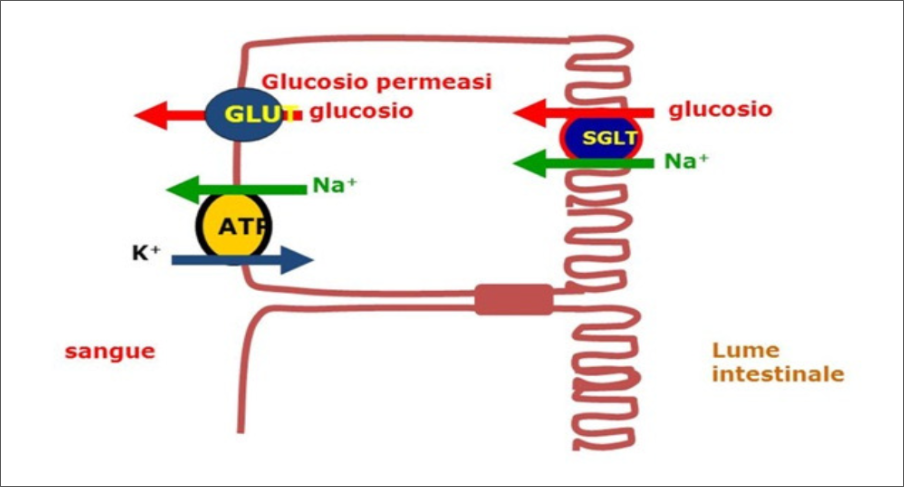
\includegraphics[width=\textwidth]{./resources/glut4.png}
    \end{figure}
    \end{center}
\end{snippet}

\begin{snippet}{glut4-expl2}
    I Glut4 verranno inseriti nella cellula quando il sangue è pieno di glucosio (quando la \textit{glicemia} è alta).
È necessario che la cellula risponda alla alta glicemia nel sangue per produrre i Glut4,
questo messaggio viene spedito attraverso il sangue con l'\textit{insulina}.
L'insulina lega il ricettore, cambiandone la struttura. \\
L'insulina viene prodotta dal pancreas, infatti, le cellule del pancreas sono in grado di misurare la glicemia.
\end{snippet}

\begin{snippet}{insulina-illustration}
    \begin{center}
    \begin{figure}[h]
        \centering
        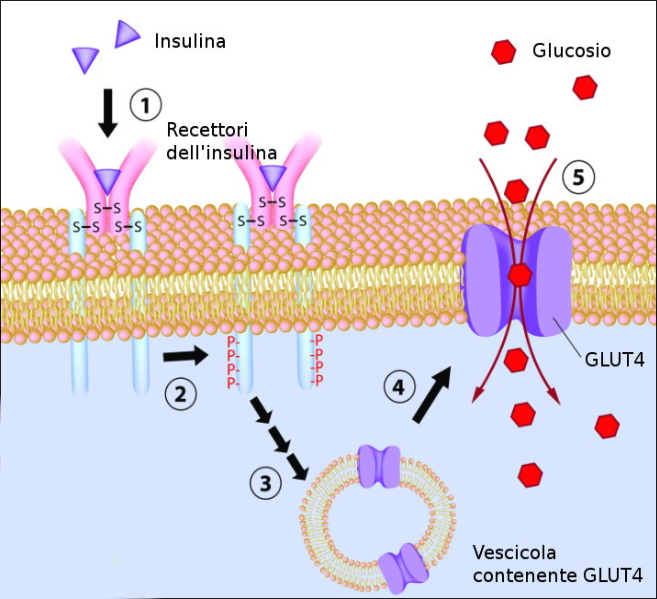
\includegraphics[width=\textwidth]{./resources/insulin.png}
    \end{figure}
    \end{center}
\end{snippet}

\plain{Il diabete è un problema nella ricezione dell'insulina.}

\begin{snippetdefinition}{omeostasi-definizione}{Omeostasi}
    L'\textit{omeostasi} è il processo di autoregolazione dei vari valori.
\end{snippetdefinition}

\plain{Il seguente diagramma illustra un esempio di omeostasi per la regolazione della glicemia nel sangue.}

\begin{snippet}{omeostasi-illustration}
    \begin{center}
    \begin{figure}[h]
        \centering
        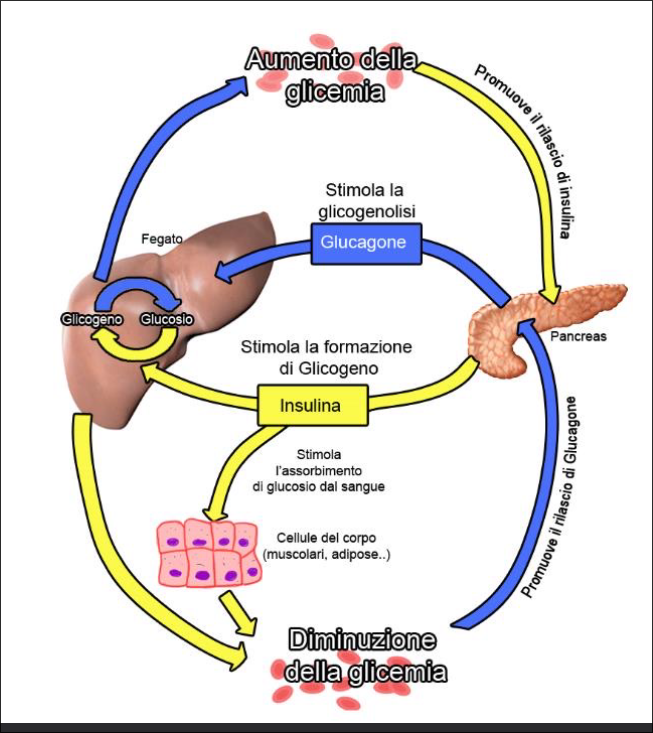
\includegraphics[width=\textwidth]{./resources/omeostasi.png}
    \end{figure}
    \end{center}
\end{snippet}

% https://tikzcd.yichuanshen.de/#N4Igdg9gJgpgziAXAbVABwnAlgFyxMJZAFgBoBGAXVJADcBDAGwFcYkQAdDnGADxwBGAM2ABBHHloQAviGml0mXPkIoAbBWp0mrdlx79hwAAr042KbPmLseAkQDMpAExaGLNok7c+OEwCcsAFt6QIgAAgAKUQAVYwBKKwUQDFsVIgBWFzcdT28DPwBlGABjAihQ-CSbZXsUMgccjz0ffmAAVTAsDH8cGTlk1NrVZCzGmnddL31fYELgnr7qlKU7EY1x7Wbp1r9RMDxF-usVtLrkDWImqZABmrXM0iuJ3PY70+GiMmetm-ehh4oAAcmhe23yswAIlghEJmNgCDBlgD0igAJzZME3GZtYpBNCMLAlJH-Vao5AAdkxvzyOL8ADF6CUsIScPQ2ciyecqZtJrTdsASvQwEwsJyziMMbzXjsCsAgjAggJ-ML6OLPvVSAAGa78gpGGIquCLMWkiVEZygmktfUiABq8GZZUYoRJJxR53I2t1NtmAFEwFAIMy+th1YDkF7XFi9f64MHcEpw+StVa+b62gBxFWBrDhND+CA8LBgN2DLkjL3S8F03DAP1wAB04Wk4TpwEzLBwxCsWhgUAA5vAiKAhIWgkhUyA+khnCcxxAJ4gpzPEA55+OkE5pxAkD3kgul9vVxkN4utzRV2oz0uNDukFSQAIYIGkABaBxam8Py+7xB359X0QD8vwPTdECye9EBBEBCVLdh40JKAQBoAALGB6GQxAwGYRhGEvegWXYSB4JoQCsKnOBUJhHAkHIb9EDIKC0QY8gVz-ch6LA89EDY386Lnbil3IS0oPIdchLor0xP3UdwPISDVynF1n0YYwK3YQIB1Q2iYwzPwAGECBwQtwmzTCsBfHhlkPOjFI4siXywz89NlWZjBgfwzJVKBLIOEkaBUmA1I0rwtJ095bN4+y6IApz30-Vi71XcgKSS-jeKBViMTEu84LyCoqP7FDp0Ixh2DZIi0IwrDpwAdwgdDMIQBjnHY2LHKAkDApLAqix4ZDAvoVT1PNLwS2wWASvTNzDBENAzAsY5JN4jK2IY48-1EmaITaOAx2YCQ1RK-L2CDCRioYmLoM6iiaComj33oyhpCAA

\begin{snippet}{schema-illustration}
    \begin{center}
    \begin{figure}[h]
        \centering
        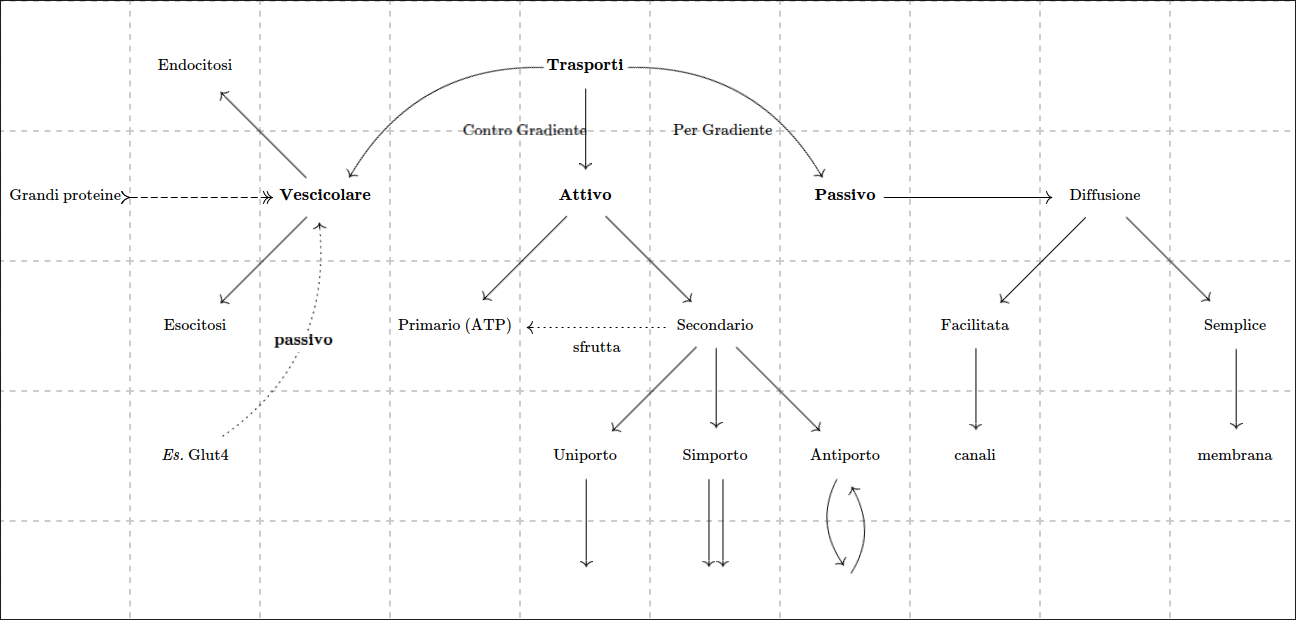
\includegraphics[width=\textwidth]{./resources/schema.png}
    \end{figure}
    \end{center}
\end{snippet}

\end{document}